\chapter{Specifikacija programske potpore}
		
	\section{Funkcionalni zahtjevi}
			
			\noindent \textbf{Dionici:}
			
			\begin{packed_enum}
				
				\item Korisnik sustava
				\begin{packed_enum}	
					\item  Maketar 
					\item  Kupac	
				\end{packed_enum}
				\item Administrator	sustava			
				\item Razvojni tim
				
			\end{packed_enum}
			
			\noindent \textbf{Aktori i njihovi funkcionalni zahtjevi:}
			
			
			\begin{packed_enum}
				\item  \underbar{Neregistrirani/neprijavljeni korisnik (inicijator) može:}
				
				\begin{packed_enum}
					
					\item registrirati se u sustav prilaganjem svoje e-mail adrese, lozinke i korisničkog imena
					\item pregledati priče i ostavljati komentare na njima
					\item unijeti podatke za kupovinu i kupiti proizvod
					\item pregledati makete i izabrati materijal makete
						
				\end{packed_enum}
					
				
				\item  \underbar{Korisnik (kupac/maketar) može:}
				
				\begin{packed_enum}
					
					\item pregledati priče i ostavljati komentare na njima
					\item pregledati makete i izabrati materijal makete
					\item slati administratoru sustava prijedloge za nove priče
					\item slati administratoru sustava zahtjev za maketu po narudžbi
					\item prihvaćati ili odbijati ponudu cijene za maketu po narudžbi
					\item vidjeti podatke o svom korisničkom računu
					\item postavljati vidljivost svojih podataka
					\item kupiti proizvod
					\item odjaviti se
					
				\end{packed_enum}
				

			
			\item  \underbar{Administrator (inicijator) može:}
			
			\begin{packed_enum}
				
				\item prihvaćati ili odbijati prijedloge priča
				\item prihvaćanjem objavljivati predložene priče
				\item ponuditi cijenu za maketu po narudžbi
				\item vidjeti podatke o izvršenim transakcijama
				\item zabraniti pristup registriranim korisnicima
				\item postavljati makete standardne ponude
				
			\end{packed_enum}
			

		
		\item  \underbar{Baza podataka (sudionik) može:}
		
		\begin{packed_enum}
			
			\item pohranjivati podatke o svim korisničkim računima sustava i njihovim ovlastima
			\item pohranjivati priče i njihove dane opise
			\item pohranjivati makete
			\item pohranjivati podatke za plaćanje
			\item pohranjivati zahtjeve za maketama
			\item pohranjivati ponude cijena za makete 
			\item pohranjivati stanje vidljivosti podataka korisnika
			\item pohranjivati podatke o izvršenim transakcijama
			\item pohranjivati podatke o korisnicima sa zabranjenim pristupom
			\item pohranjivati podatke maketa standardne ponude 
			
		\end{packed_enum}
		\end{packed_enum}
			
			\eject 
			
			
				
			\subsection{Obrasci uporabe}
				
				\subsubsection{Opis obrazaca uporabe}
							
						\noindent \underbar{\textbf{UC1 $-$ Registracija}}
					\begin{packed_item}
						
						\item \textbf{Glavni sudionik: }Korisnik
						\item  \textbf{Cilj:} Napraviti korisnički račun za korisnika
						\item  \textbf{Sudionici:} Baza podataka
						\item  \textbf{Preduvjet:} -
						\item  \textbf{Opis osnovnog tijeka:}
						
						\item[] \begin{packed_enum}
							
							\item Neregistrirani korisnik odabire opciju za registraciju
							\item Unosi potrebne podatke za registraciju
							\item Korisnikovi podaci se upisuju u bazu te je obaviješten o uspješnoj registraciji
						\end{packed_enum}
						
						\item  \textbf{Opis mogućih odstupanja:}
						
						\item[] \begin{packed_item}
							
							\item[2.a] Odabir već zauzetog korsiničkog imena i/ili e-maila, unos podataka u nedozvoljenom formatu (npr. lozinka) ili pružanje neispravnog e-maila
							\item[] \begin{packed_enum}
								
								\item Korisnik je obaviješten o nastaloj grešci i mjestu na kojem se ona nalazi
								\item Korisnik potom ispravlja grešku i ponovo šalje podatke ili odustaje od registracije
								
							\end{packed_enum}					
						\end{packed_item}
					\end{packed_item}
				
						\noindent \underbar{\textbf{UC2 $-$ Pregled priča}}
					\begin{packed_item}
						
						\item \textbf{Glavni sudionik: }Korisnik
						\item  \textbf{Cilj:} Korisniku se pruža stranica sa kratkim prikazom svih priča u sustavu
						\item  \textbf{Sudionici:} Baza podataka
						\item  \textbf{Preduvjet:} -
						\item  \textbf{Opis osnovnog tijeka:}
						
						\item[] \begin{packed_enum}
							
							\item Korisnik sa početne stranice poveznicom dolazi do stranice sa pričama
							\item Aplikacija korisniku prikazuje sve priče u sustavu
						\end{packed_enum}
					\end{packed_item}
				
						\noindent \underbar{\textbf{UC3 $-$ Pregled pojedine priče}}
					\begin{packed_item}
						
						\item \textbf{Glavni sudionik: }Korisnik
						\item  \textbf{Cilj:} Korisniku se pruža detaljan prikaz određene priče
						\item  \textbf{Sudionici:} Baza podataka
						\item  \textbf{Preduvjet:} -
						\item  \textbf{Opis osnovnog tijeka:}
						
						\item[] \begin{packed_enum}
							
							\item Korisnik iz kratkog prikaza priča odabire priču koja ga zanima
							\item Aplikacija korisniku pruža detaljan prikaz priče (slika, video, tekst) i mogućnost komentiranja na priču
						\end{packed_enum}
					\end{packed_item}
				
						\noindent \underbar{\textbf{UC4 $-$ Komentiranje priče}}
					\begin{packed_item}
						
						\item \textbf{Glavni sudionik: }Korisnik
						\item  \textbf{Cilj:} Korisnik sustava ostavlja komentar na priču 
						\item  \textbf{Sudionici:} Baza podataka
						\item  \textbf{Preduvjet:} -
						\item  \textbf{Opis osnovnog tijeka:}
						
						\item[] \begin{packed_enum}
							\item Korisnik otvara priču na kojoj želi ostaviti komentar
							\item U za to namijenjeno mjesto upisuje komentar te ga objavljuje
							\item Komentar se objavljuje te je uz njega navedeno ime korisnika koji ga je objavio
							\item 
						\end{packed_enum}
						
						\item  \textbf{Opis mogućih odstupanja:}
						
						\item[] \begin{packed_item}
							
							\item[3.a] Korisnik nije prijavljen u sustav
							\item[] \begin{packed_enum}
								
								\item Umjesto korisničkog imena na to mjesto se upisuje $"$Anoniman korisnik$"$
								
							\end{packed_enum}
							\item[2.b] $<$opis mogućeg scenarija odstupanja u koraku 2$>$
							\item[3.a] $<$opis mogućeg scenarija odstupanja  u koraku 3$>$
							
						\end{packed_item}
					\end{packed_item}
				
						\noindent \underbar{\textbf{UC5 $-$ Predlaganje priče}}
					\begin{packed_item}
						
						\item \textbf{Glavni sudionik: }Korisnik
						\item  \textbf{Cilj:} Korisnik šalje prijedlog priče za objavu na stranici administratoru 
						\item  \textbf{Sudionici:} Administrator, baza podataka
						\item  \textbf{Preduvjet:} Korisnik je prijavljen u sustav
						\item  \textbf{Opis osnovnog tijeka:}
						
						\item[] \begin{packed_enum}
							
							\item Korisnik iz izbornika odabire opciju predlaganja priče
							\item Aplikacija mu pruža sučelje za dodavanje opisa priče (slika, video, tekst)
							\item Korisnik popunjava podatke i šalje ih administratoru na pregled
						\end{packed_enum}
						
						\item  \textbf{Opis mogućih odstupanja:}
						
						\item[] \begin{packed_item}
							
							\item[2.a] Korisnik nije predao dovoljno podataka (nema ni slike, ni teksta, ni videa i/ili nema naslova) 
							\item[] \begin{packed_enum}
								
								\item Korisnik je obaviješten o grešci i mjestu na kojem je nastala
								\item Korisnik ispravlja grešku i šalje podatke administratoru na pregled ili odustaje od slanja prijedloga priče								
							\end{packed_enum}			
						\end{packed_item}
					\end{packed_item}
				
					\noindent \underbar{\textbf{UC6 $-$ Prilaganje slike/teksta/videa priči}}
				\begin{packed_item}
					
					\item \textbf{Glavni sudionik: }Korisnik
					\item  \textbf{Cilj:} Opisivanje priče koja se predlaže administratoru tekstom, slikom i videom
					\item  \textbf{Sudionici:} Baza podataka
					\item  \textbf{Preduvjet:} Korisnik je prijavljen u sustav
					\item  \textbf{Opis osnovnog tijeka:}
					
					\item[] \begin{packed_enum}
						
						\item Korisniku je pružen upravljač kojim dodaje proizvoljan broj elemenata teksta, slike i videa 
						\item Korisnik u elemente upisuje tekst ili prilaže sliku ili video ili ih uklanja
						\item Nakon što je popunio podatke, može ih slati administratoru
					\end{packed_enum}
					
					\item  \textbf{Opis mogućih odstupanja:}
					
					\item[] \begin{packed_item}
						
						\item[2.a] Korisnik prilaže sliku ili video nedozvoljenog formata
						\item[] \begin{packed_enum}
							
							\item Korisnik je obaviješten o grešci i dano mu je pojašnjenje te greške
							\item Korisnik odustaje od prilaganja slike/videa uz priču ili prilaže sliku/video u drugom formatu
							
						\end{packed_enum}	
					\end{packed_item}
				\end{packed_item}
			
					\noindent \underbar{\textbf{UC7 $-$ Odobrenje/odbijanje priče}}
				\begin{packed_item}
					
					\item \textbf{Glavni sudionik: }Administrator
					\item  \textbf{Cilj:} Predložena priča se objavljuje na za to predviđenoj stranici ili se odbacuje
					\item  \textbf{Sudionici:} Baza podataka
					\item  \textbf{Preduvjet:} Korisnik je prijavljen i dodana su mu prava administratora
					\item  \textbf{Opis osnovnog tijeka:}
					
					\item[] \begin{packed_enum}
						
						\item Aplikacija administratoru pruža listu priča danih na prijedlog i njihov opis
						\item Administratoru je ispod svake priče ponuđena opcija odbacivanja ili prihvaćanja priče
						\item Priča se ovisno o administratorovom izboru uklanja iz sustava ili se objavljuje
					\end{packed_enum}
				\end{packed_item}
			
					\noindent \underbar{\textbf{UC8 $-$ Objava priče}}
				\begin{packed_item}
					
					\item \textbf{Glavni sudionik: }Administrator
					\item  \textbf{Cilj:} Priča se nakon administratorovog odobravanja prikazuje svim korisnicima sustava na za to određenom mjestu
					\item  \textbf{Sudionici:} Baza podataka
					\item  \textbf{Preduvjet:} Korisnik je prijavljen u sustav i dodana su mu prava administratora
					\item  \textbf{Opis osnovnog tijeka:}
					
					\item[] \begin{packed_enum}
						
						\item Administrator prihvaća priču
						\item Priča se pohranjuje u bazu podataka te se prikazuje na određenoj stranici zajedno sa ostalim pričama
					\end{packed_enum}
				\end{packed_item}
				
					\noindent \underbar{\textbf{UC9 $-$ Prijava}}
				\begin{packed_item}
					
					\item \textbf{Glavni sudionik: }Korisnik
					\item  \textbf{Cilj:} Prijaviti korisnika u sustav
					\item  \textbf{Sudionici:} Baza podataka
					\item  \textbf{Preduvjet:} Korisnik je registriran u bazi podataka
					\item  \textbf{Opis osnovnog tijeka:}
						
					\item[] \begin{packed_enum}
							
						\item Neprijavljen korisnik odabire opciju za prijavu
						\item Unosi potrebne podatke za prijavu
						\item Podaci se provjeravaju u bazi podataka te se obavještava o uspješnoj prijavi
					\end{packed_enum}
						
					\item  \textbf{Opis mogućih odstupanja:}
						
					\item[] \begin{packed_item}
							
						\item[2.a] Unos nepostojećeg korisničkog imena ili e-maila, unos pogrešne lozinke
						\item[] \begin{packed_enum}
								
							\item Korisnik je obaviješten o nastaloj grešci i mjestu na kojem se ona nalazi
							\item Korisnik potom ispravlja grešku i ponovo šalje podatke ili odustaje od prijave
								
						\end{packed_enum}					
					\end{packed_item}
				\end{packed_item}
				
					\noindent \underbar{\textbf{UC10 $-$ Odjava}}
				\begin{packed_item}
					
					\item \textbf{Glavni sudionik: }Korisnik
					\item  \textbf{Cilj:} Odjaviti se iz sustava
					\item  \textbf{Sudionici:} -
					\item  \textbf{Preduvjet:} Korisnik je prijavljen u sustav
					\item  \textbf{Opis osnovnog tijeka:}
					
					\item[] \begin{packed_enum}
						
						\item Prijavljen korisnik odabire opciju za odjavu 
						\item Obavještava se korisnika o uspješnoj odjavi
					\end{packed_enum}
				\end{packed_item}
				
					\noindent \underbar{\textbf{UC11 $-$ Prikaz korisničkog računa}}
				\begin{packed_item}
					
					\item \textbf{Glavni sudionik: }Korisnik
					\item  \textbf{Cilj:} Prikazati podatke o korisničkom računu
					\item  \textbf{Sudionici:} Baza podataka
					\item  \textbf{Preduvjet:} Korisnik je prijavljen u sustav
					\item  \textbf{Opis osnovnog tijeka:}
					
					\item[] \begin{packed_enum}
						
						\item Prijavljen korisnik odabire opciju za prikaz svog korisničkog računa 
						\item Prikazuju se podaci o korisničkom računu
					\end{packed_enum}
				\end{packed_item}
				
					\noindent \underbar{\textbf{UC12 $-$ Unos podataka za kupovinu za prijavljenog korisnika}}
				\begin{packed_item}
					
					\item \textbf{Glavni sudionik: }Korisnik
					\item  \textbf{Cilj:} Popuniti formular za kupovinu makete
					\item  \textbf{Sudionici:} Baza podataka
					\item  \textbf{Preduvjet:} Korisnik je prijavljen u bazi podataka
					\item  \textbf{Opis osnovnog tijeka:}
						
					\item[] \begin{packed_enum}
							
						\item Prijavljen korisnik odabire opciju za kupnju makete
						\item Formular s podacima za kupovinu se automatski ispuni osobnim podacima
						\item Odabire se opcija za izvršavanje transakcije/kupnje
						\item Obavještava se korisnika o uspješnoj transakciji/kupnji
					\end{packed_enum}
				\end{packed_item}
				
					\noindent \underbar{\textbf{UC13 $-$ Unos podataka za kupovinu za neregistriranog korisnika}}
				\begin{packed_item}
					
					\item \textbf{Glavni sudionik: }Korisnik
					\item  \textbf{Cilj:} Popuniti formular za kupovinu makete
					\item  \textbf{Sudionici:} Baza podataka
					\item  \textbf{Preduvjet:} -
					\item  \textbf{Opis osnovnog tijeka:}
						
					\item[] \begin{packed_enum}
							
						\item Neregistrirani korisnik odabire opciju za kupnju makete
						\item Ispunjava formular za kupovinu s osobnim podacima
						\item Odabire se opcija za izvršavanje transakcije/kupnje
						\item Obavještava se korisnika o uspješnoj transakciji/kupnji
					\end{packed_enum}
						
					\item  \textbf{Opis mogućih odstupanja:}
						
					\item[] \begin{packed_item}
							
						\item[2.a] Unos pogrešnih osobnih podataka ili podataka potrebnih za transakciju
						\item[] \begin{packed_enum}
								
							\item Korisnik je obaviješten o nastaloj grešci i mjestu na kojem se ona nalazi
							\item Korisnik potom ispravlja grešku i ponovo šalje podatke ili odustaje od kupnje
								
						\end{packed_enum}					
					\end{packed_item}
				\end{packed_item}
				
					\noindent \underbar{\textbf{UC14 $-$ Spremanje izvršenih transakcija}}
				\begin{packed_item}
					
					\item \textbf{Glavni sudionik: }Baza podataka
					\item  \textbf{Cilj:} Spremiti izvršene transakcije u bazu podataka
					\item  \textbf{Sudionici:} -
					\item  \textbf{Preduvjet:} Transakcija je uspješno obavljena
					\item  \textbf{Opis osnovnog tijeka:}
						
					\item[] \begin{packed_enum}
							
						\item Sustav javlja korisniku da je transakcija uspješna
						\item Baza podataka sprema podatke o transakciji
					\end{packed_enum}
				\end{packed_item}
				
					\noindent \underbar{\textbf{UC15 $-$ Pregled izvršenih transakcija}}
				\begin{packed_item}
					
					\item \textbf{Glavni sudionik: }Administrator
					\item  \textbf{Cilj:} Pregled podataka o izvršenim transakcijama
					\item  \textbf{Sudionici:} Baza podataka
					\item  \textbf{Preduvjet:} Korisnik je prijavljen u sustav i dodana su mu prava administratora
					\item  \textbf{Opis osnovnog tijeka:}
						
					\item[] \begin{packed_enum}
							
						\item Administrator odabire opciju za pregled prošlih transakcija
						\item Prikazuju se podaci iz baze podataka o transakcijama
					\end{packed_enum}
				\end{packed_item}
			
					\noindent \underbar{\textbf{UC16 $-$ Pregled maketa}}
				\begin{packed_item}
				
					\item \textbf{Glavni sudionik: }Korisnik
					\item  \textbf{Cilj:} Korisniku se pruža stranica s kratkim prikazom svih maketa u sustavu
					\item  \textbf{Sudionici:} Baza podataka
					\item  \textbf{Preduvjet:} -
					\item  \textbf{Opis osnovnog tijeka:}
					
					\item[] \begin{packed_enum}
					
						\item Korisnik s početne stranice poveznicom dolazi do stranice s maketama
						\item Aplikacija korisniku prikazuje sve makete u sustavu
					\end{packed_enum}
				\end{packed_item}
			
			
					\noindent \underbar{\textbf{UC17 $-$ Pregled pojedine makete}}
				\begin{packed_item}
					
					\item \textbf{Glavni sudionik: }Korisnik
					\item  \textbf{Cilj:} Korisniku se pruža detaljan prikaz pojedine makete
					\item  \textbf{Sudionici:} Baza podataka
					\item  \textbf{Preduvjet:} -
					\item  \textbf{Opis osnovnog tijeka:}
					
					\item[] \begin{packed_enum}
						
						\item Korisnik sa stranice s pregledom svih maketa odabire maketu koja ga zanima
						\item Aplikacija korisniku prikazuje detaljan opis tražene makete koji uključuje tekst, slike, izbornike te mogućnost kupovine makete
					\end{packed_enum}
				\end{packed_item}
			
				\noindent \underbar{\textbf{UC18 $-$ Odabir materijala za maketu}}
				\begin{packed_item}
					
					\item \textbf{Glavni sudionik: }Korisnik
					\item  \textbf{Cilj:} Korisniku se pruža mogućnost odabira materijala od kojeg želi da se izradi maketa
					\item  \textbf{Sudionici:} Baza podataka
					\item  \textbf{Preduvjet:} Korisnik mora biti na stranici pojedinačne makete
					\item  \textbf{Opis osnovnog tijeka:}
					
					\item[] \begin{packed_enum}
						
						\item Korisnik na stranici makete otvara padajući izbornik s opcijama za materijale te odabire željeni materijal
						\item Aplikacija na osnovu odabranog materijala izračunava cijenu makete te prikazuje novu cijenu na stranici
					\end{packed_enum}
				\end{packed_item}
				
				
				\noindent \underbar{\textbf{UC19 $-$ Spremanje podataka formulara za plaćanje}}
				\begin{packed_item}
					
					\item \textbf{Glavni sudionik: }Korisnik
					\item  \textbf{Cilj:} Formular koji je ispunio registrirani korisnik pri plaćanju se sprema za ponovno korištenje
					\item  \textbf{Sudionici:} Baza podataka
					\item  \textbf{Preduvjet:} Korisnik mora biti registriran te ispravno popuniti formular
					\item  \textbf{Opis osnovnog tijeka:}
					
					\item[] \begin{packed_enum}
						
						\item Korisnik na stranici za plaćanje ispunjava formular
						\item Aplikacija provjerava ispravnost unesenih podataka
						\item Nakon provjere podatci se spremaju u bazu podataka za ponovnu upotrebu pri sljedećoj kupovini
					\end{packed_enum}
				
					\item  \textbf{Opis mogućih odstupanja:}
					
					\item[] \begin{packed_item}
						
						\item[2.a] Korisnik neispravno popuni jedno ili više polja ili ostavi prazno polje
						\item[] \begin{packed_enum}
							
							\item Korisnik je obaviješten o grešci i dano mu je pojašnjenje te greške
							\item Korisnik prepravlja ili nadopunjava podatke te se oni ponovno šalju na validaciju ili odustaje od ispunjavanja formulara
							
						\end{packed_enum}	
					\end{packed_item}
				\end{packed_item}
			
				\noindent \underbar{\textbf{UC20 $-$ Popunjavanje formulara za maketu po narudžbi}}
				\begin{packed_item}
					
					\item \textbf{Glavni sudionik: }Korisnik
					\item  \textbf{Cilj:} Korisnik predaje formular sa specifikacijama željene makete 
					\item  \textbf{Sudionici:} Baza podataka, administrator
					\item  \textbf{Preduvjet:} Korisnik mora biti registriran te ispravno popuniti formular
					\item  \textbf{Opis osnovnog tijeka:}
					
					\item[] \begin{packed_enum}
						
						\item Korisnik na stranici za ispunjavanje formulara popunjava formular sa željenim dimenzijama, materijalom i opisom
						\item Aplikacija provjerava ispravnost unesenih podataka
						\item Nakon provjere podatci se spremaju u bazu podataka
						\item Administratoru se šalje obavijest o novom formularu
					\end{packed_enum}
					
					\item  \textbf{Opis mogućih odstupanja:}
					
					\item[] \begin{packed_item}
 
						\item[2.a] Korisnik neispravno popuni jedno ili više polja ili ostavi prazno polje
						\item[] \begin{packed_enum}
							
							\item Korisnik je obaviješten o grešci i dano mu je pojašnjenje te greške
							\item Korisnik prepravlja ili nadopunjava podatke te se oni ponovno šalju na validaciju ili odustaje od ispunjavanja formulara
							
						\end{packed_enum}	
					\end{packed_item}
				\end{packed_item}


				\noindent \underbar{\textbf{UC21 $-$ Ponuda makete na zahtjev}}
				\begin{packed_item}
					
					\item \textbf{Glavni sudionik: }Administrator
					\item  \textbf{Cilj:} Administrator pregledava zahtjev te šalje ponudu na osnovu traženih specifikacija
					\item  \textbf{Sudionici:} Baza podataka, korisnik
					\item  \textbf{Preduvjet:} Administrator mora imati predan zahtjev od strane korisnika
					\item  \textbf{Opis osnovnog tijeka:}
					
					\item[] \begin{packed_enum}
						
						\item Administrator dobija obavijest o podnesenom zahtjevu te otvara zahtjev
						\item Administrator na osnovu zahtjeva određuje cijenu te šalje ponudu korisniku
						\item Korisnik dobija obavijest o ponudi
					\end{packed_enum}
				\end{packed_item}

				\noindent \underbar{\textbf{UC22 $-$ Prihvat ili odbijanje ponude makete}}
				\begin{packed_item}
					
					\item \textbf{Glavni sudionik: }Korisnik
					\item  \textbf{Cilj:} Korisnik prihvaća ili odbija ponuđenu cijenu makete
					\item  \textbf{Sudionici:} Baza podataka, administrator
					\item  \textbf{Preduvjet:} Korisnik mora biti registriran
					\item  \textbf{Opis osnovnog tijeka:}
					
					\item[] \begin{packed_enum}
						
						\item Korisnik dobija obavijest o ponudi cijene za maketu
						\item Korisnik odbija ili prihvaća ponudu
						\item Šalje se povratna informacija administratoru
					\end{packed_enum}
				\end{packed_item}

				\noindent \underbar{\textbf{UC23 $-$ Postavljanje postavki vidljivosti korisničkog računa}}
				\begin{packed_item}
					
					\item \textbf{Glavni sudionik: }Korisnik
					\item  \textbf{Cilj:} Korisnik postavlja željenu vidljivost svojih podataka
					\item  \textbf{Sudionici:} Baza podataka
					\item  \textbf{Preduvjet:} Korisnik mora biti registriran
					\item  \textbf{Opis osnovnog tijeka:}
					
					\item[] \begin{packed_enum}
						
						\item Korisnik odabire stranicu s postavkama korisničkog računa
						\item Korisnik odabire opciju postavljanja vidljivosti
						\item Korisnik odabire stavke koje želi da budu privatne ili javne (korisničko ime mora biti javno)
						\item Korisnik potvrđuje odabir te se on šalje sustavu
						\item Stranica osvježava podatke
					\end{packed_enum}

					\item  \textbf{Opis mogućih odstupanja:}
					
					\item[] \begin{packed_item}
 
						\item[4.a] Korisnik ne potvrdi svoj odabir prije napuštanja stranice
						\item[] \begin{packed_enum}
							
							\item Korisnik je obaviješten o grešci te se nudi opcija povratka na potvrdu odabira
							\item Korisnik potvrđuje ili odustaje od izmjena
							
						\end{packed_enum}	
					\end{packed_item}
				\end{packed_item}

				\noindent \underbar{\textbf{UC24 $-$ Zabrana pristupa korisniku}}
				\begin{packed_item}
					
					\item \textbf{Glavni sudionik: }Administrator
					\item  \textbf{Cilj:} Administrator zabranjuje pristup određenom registriranom korisniku
					\item  \textbf{Sudionici:} Baza podataka, korisnik
					\item  \textbf{Preduvjet:} Korisnik mora biti registriran
					\item  \textbf{Opis osnovnog tijeka:}
					
					\item[] \begin{packed_enum}
						
						\item Administrator odabire korisnika kojem želi zabraniti pristup
						\item Potvrđuje odabir te se sprema u bazu podataka
					\end{packed_enum}
				\end{packed_item}


				\noindent \underbar{\textbf{UC25 $-$ Kreiranje standardne ponude maketa}}
				\begin{packed_item}
					
					\item \textbf{Glavni sudionik: }Administrator
					\item  \textbf{Cilj:} Administrator ispunjava i objavljuje standardnu ponudu na stranici
					\item  \textbf{Sudionici:} Baza podataka
					\item  \textbf{Preduvjet:} -
					\item  \textbf{Opis osnovnog tijeka:}
					
					\item[] \begin{packed_enum}
						
						\item Administrator ispunjava podatke za novu ponudu makete
						\item Administrator potvrđuje formular te se šalje u bazu podataka
						\item Nova maketa se sprema te se počinje prikazivati na stranici
					\end{packed_enum}

					\item  \textbf{Opis mogućih odstupanja:}
					
					\item[] \begin{packed_item}
 
						\item[2.a] Administrator krivo ispuni ili ostavi prazno polje u formularu
						\item[] \begin{packed_enum}
							
							\item Administrator je obaviješten o grešci te se nudi opcija povratka na ispunjavanje formulara
							\item Korisnik izmjenjuje ili nadopunjava podatke te ponovno potvrđuje odabir
							
						\end{packed_enum}	
					\end{packed_item}
				\end{packed_item}
			
			\noindent \underbar{\textbf{UC26 $-$ Kupnja makete}}
			\begin{packed_item}
				
				\item \textbf{Glavni sudionik: }Korisnik
				\item  \textbf{Cilj:} Korisniku se nudi obrazac koji služi za popunjavanje podataka potrebnih za kupnju
				\item  \textbf{Sudionici:} Baza podataka
				\item  \textbf{Preduvjet:} -
				\item  \textbf{Opis osnovnog tijeka:}
				
				\item[] \begin{packed_enum}
					
					\item Korisnik sa stranice makete odabire opciju kupnje nje
					\item Korisniku se prikazuje obrazac u kojem popunjava ili provjerava podatke za kupnju
				\end{packed_enum}
			\end{packed_item}
					
				\subsubsection{Dijagrami obrazaca uporabe}
					
					\begin{figure}[H]
						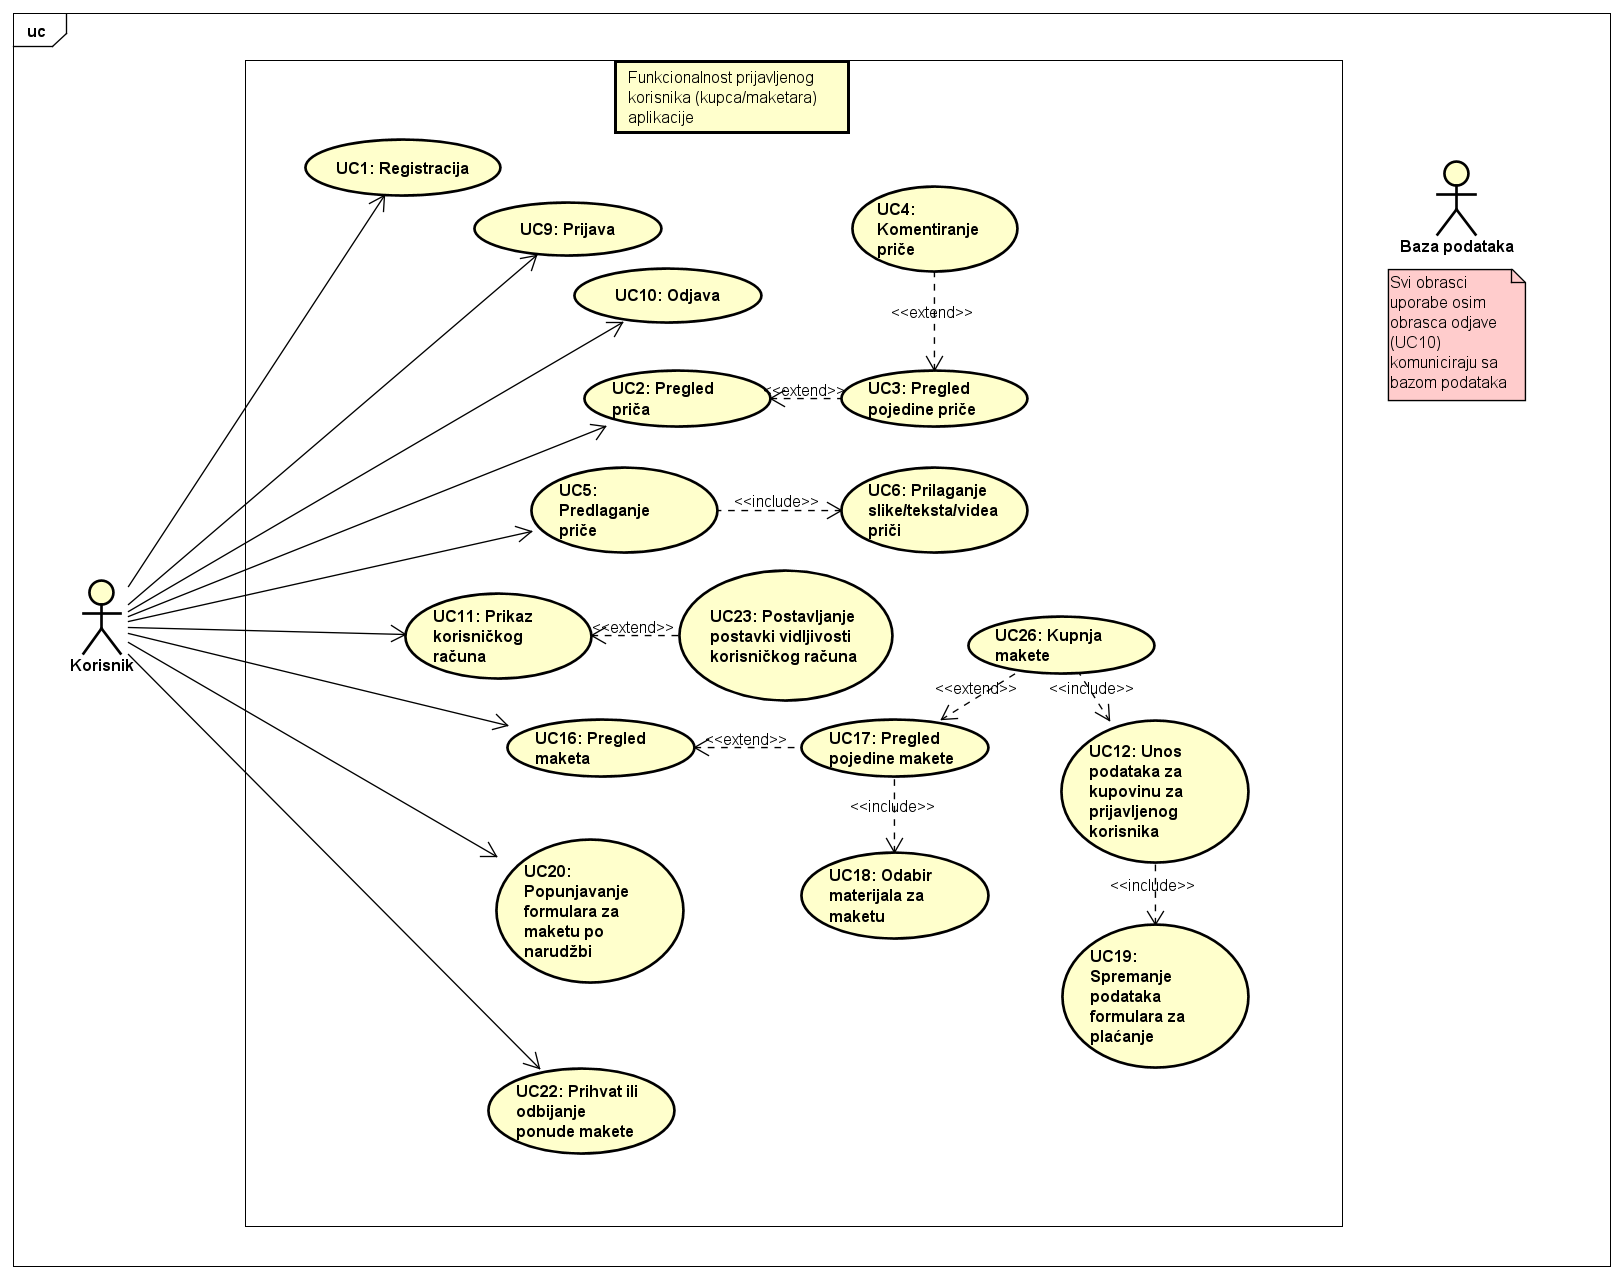
\includegraphics[width=.9\linewidth]{slike/Funkcionalnost_prijavljenog_korisnika.PNG} %veličina u odnosu na širinu linije
						\caption{Dijagram obrasca uporabe, funkcionalnost prijavljenog korisnika}
						\label{fig:obrupo1} %label mora biti drugaciji za svaku sliku
					\end{figure}

					\begin{figure}[H]
						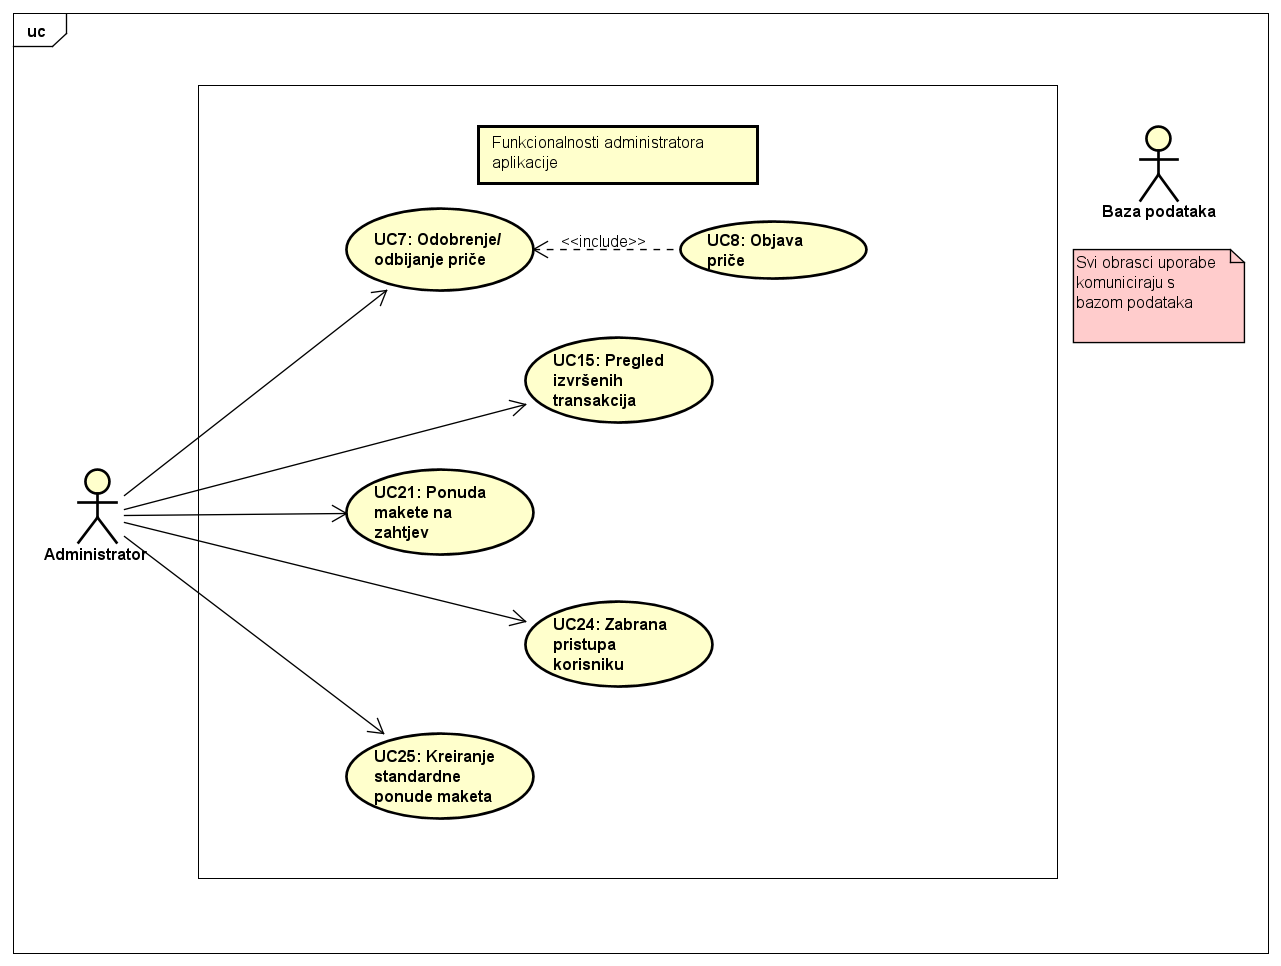
\includegraphics[width=.9\linewidth]{slike/Funkcionalnost_administratora_sustava.PNG} %veličina u odnosu na širinu linije
						\caption{Dijagram obrasca uporabe, funkcionalnost administratora}
						\label{fig:obrupo2} %label mora biti drugaciji za svaku sliku
					\end{figure}

				\eject		
				
			\subsection{Sekvencijski dijagrami}
				
				\textbf{\textit{dio 1. revizije}}\\
				
				\textit{Nacrtati sekvencijske dijagrame koji modeliraju najvažnije dijelove sustava (max. 4 dijagrama). Ukoliko postoji nedoumica oko odabira, razjasniti s asistentom. Uz svaki dijagram napisati detaljni opis dijagrama.}
				\eject
	
		\section{Ostali zahtjevi}
		
			\textbf{\textit{dio 1. revizije}}\\
		 
			 \textit{Nefunkcionalni zahtjevi i zahtjevi domene primjene dopunjuju funkcionalne zahtjeve. Oni opisuju \textbf{kako se sustav treba ponašati} i koja \textbf{ograničenja} treba poštivati (performanse, korisničko iskustvo, pouzdanost, standardi kvalitete, sigurnost...). Primjeri takvih zahtjeva u Vašem projektu mogu biti: podržani jezici korisničkog sučelja, vrijeme odziva, najveći mogući podržani broj korisnika, podržane web/mobilne platforme, razina zaštite (protokoli komunikacije, kriptiranje...)... Svaki takav zahtjev potrebno je navesti u jednoj ili dvije rečenice.}
			 
			 
			 
	